\chapter{Cinematica}

\subsection{Grandezze scalari e vettoriali}

\textbf{Grandezza scalare}: è completamente definita da un valore numerico e dall'unità di misura.

\noindent\textbf{Grandezza vettoriale}: è definita da modulo, direzione e verso.

\noindent\textbf{Versore}: vettore di modulo unitario utilizzato per indicare una direzione.

\[
|\hat{i}|=|\hat{j}|=|\hat{k}|=1
\]

\vspace{0.3cm}

\subsection{Posizione e spostamento}

Vettore posizione:

\[
\vec{r}=x\hat{i}+y\hat{j}+z\hat{k}
\]

\noindent Lo spostamento è il vettore che unisce la posizione iniziale con quella finale:

\[
\Delta \vec{r}=\vec{r}_f-\vec{r}_i
\]

\noindent\textbf{Attenzione}

\noindent Lo spazio percorso è la lunghezza totale della traiettoria.

\noindent Lo spostamento dipende solamente dalla posizione iniziale e finale.

\vspace{0.3cm}

\subsection{Velocità}

Velocità scalare media:

\[
v_m=\frac{\Delta s}{\Delta t}
\]

\noindent Misura quanto spazio viene percorso nell'unità di tempo.

\noindent Velocità vettoriale media:

\[
\vec{v}_m=\frac{\Delta \vec{r}}{\Delta t}
\]

\noindent Tiene conto anche della direzione del moto.

\vspace{0.3cm}

\subsection{Accelerazione}

Accelerazione media:

\[
a=\frac{\Delta v}{\Delta t}
\]

\noindent Misura la variazione della velocità nel tempo.

\begin{itemize}
\item $a>0$: la velocità aumenta (nel verso positivo scelto).
\item $a<0$: la velocità diminuisce se ha lo stesso verso dell'accelerazione, oppure aumenta nel verso opposto.
\item $a=0$: velocità costante.
\end{itemize}

\vspace{0.3cm}

\subsection{Moto Rettilineo Uniforme (MRU)}

Condizioni:

\begin{itemize}
\item traiettoria rettilinea;
\item velocità costante;
\item accelerazione nulla.
\end{itemize}

\noindent Legge oraria:

\[
s=s_0+vt
\]

\noindent dove:

\begin{itemize}
\item $s_0$ posizione iniziale;
\item $v$ velocità costante;
\item $t$ tempo.
\end{itemize}

\vspace{0.3cm}

\subsection{Moto Rettilineo Uniformemente Accelerato (MUA)}

Condizioni:

\begin{itemize}
\item traiettoria rettilinea;
\item accelerazione costante.
\end{itemize}

\noindent Velocità:

\[
v=v_0+at
\]

\noindent Posizione:

\[
s=s_0+v_0t+\frac{1}{2}at^2
\]

\noindent Relazione indipendente dal tempo:

\[
v^2=v_0^2+2a(s-s_0)
\]

\vspace{0.3cm}

\subsection{Caduta libera}

La caduta libera è un caso particolare di MUA.

\noindent L'accelerazione è costante e pari a:

\[
g=9.81\,\mathrm{m/s^2}
\]

\noindent Le formule diventano:

\[
v=v_0+gt
\]

\[
s=s_0+v_0t+\frac{1}{2}gt^2
\]

\[
v^2=v_0^2+2g(s-s_0)
\]

\textbf{Nota}

Il segno di $g$ dipende dal sistema di riferimento scelto.

\vspace{0.3cm}

\subsection{Lancio verticale}

Nel punto più alto:

\[
v=0
\]

\noindent ma:

\[
a=-g
\]

\noindent L'accelerazione non diventa mai nulla.

\vspace{0.3cm}

\subsection{Moto parabolico}

È la composizione di due moti indipendenti.

\noindent Asse orizzontale (Asse x):

\[
\text{MRU}
\]

\noindent Asse verticale (Asse y):

\[
\text{MUA}
\]

\noindent I due moti vengono studiati separatamente.

\vspace{0.3cm}

\subsection{Moto circolare uniforme}

La velocità mantiene modulo costante ma cambia continuamente direzione.

\noindent Accelerazione centripeta:

\[
a_c=\frac{v^2}{r}
\]

\noindent dove:

\begin{itemize}
\item $a_c$: accelerazione centripeta;
\item $v$: velocità del corpo;
\item $r$: raggio della traiettoria circolare.
\end{itemize}

\vspace{0.2cm}

\noindent Forza centripeta:

\[
F_c=m\frac{v^2}{r}
\]

\noindent dove:

\begin{itemize}
\item $F_c$: forza centripeta;
\item $m$: massa del corpo;
\item $v$: velocità del corpo;
\item $r$: raggio della traiettoria circolare.
\end{itemize}

\noindent La forza è sempre diretta verso il centro della traiettoria.

\vspace{0.3cm}

\subsection{Moto armonico}

Legge di Hooke:

\[
F=-kx
\]

\noindent dove:

\begin{itemize}
\item $F$: forza elastica esercitata dalla molla;
\item $k$: costante elastica della molla;
\item $x$: spostamento dalla posizione di equilibrio.
\end{itemize}

\noindent Il segno meno indica che la forza è sempre diretta verso la posizione di equilibrio.

\vspace{0.2cm}

\noindent Periodo della molla:

\[
T=2\pi\sqrt{\frac{m}{k}}
\]

\noindent dove:

\begin{itemize}
\item $T$: periodo dell'oscillazione (tempo necessario per compiere un'oscillazione completa);
\item $m$: massa collegata alla molla;
\item $k$: costante elastica della molla.
\end{itemize}

\vspace{0.2cm}

\noindent Periodo del pendolo semplice (piccole oscillazioni):

\[
T=2\pi\sqrt{\frac{l}{g}}
\]

\noindent dove:

\begin{itemize}
\item $T$: periodo dell'oscillazione;
\item $l$: lunghezza del filo del pendolo;
\item $g$: accelerazione di gravità.
\end{itemize}
\chapter{Dinamica}
\subsection{Seconda legge di Newton}

\[
\boxed{\sum \vec{F}=m\vec{a}}
\]

\noindent La risultante delle forze agenti su un corpo è uguale al prodotto tra massa e accelerazione.

\noindent con:

\begin{itemize}
    \item $\sum \vec{F}$ = risultante delle forze;
    \item $m$ = massa del corpo;
    \item $\vec{a}$ = accelerazione.
\end{itemize}

\vspace{0.3cm}

\subsection{Peso}

\[
\boxed{P=mg}
\]

\noindent Il peso è la forza con cui la Terra attrae un corpo.

\noindent con:

\begin{itemize}
    \item $P$ = peso;
    \item $m$ = massa;
    \item $g$ = accelerazione di gravità ($9.81\,m/s^2$).
\end{itemize}

\noindent Il peso è sempre diretto verticalmente verso il basso.

\vspace{0.3cm}

\subsection{Reazione normale}

\noindent Su un piano orizzontale:

\[
\boxed{N=P=mg}
\]

\noindent Su un piano inclinato:

\[
\boxed{N=mg\cos\theta}
\]

\noindent con:

\begin{itemize}
    \item $N$ = reazione normale;
    \item $m$ = massa;
    \item $g$ = accelerazione di gravità;
    \item $\theta$ = angolo di inclinazione del piano.
\end{itemize}

\noindent La reazione normale è sempre perpendicolare alla superficie di contatto.

\vspace{0.3cm}

\subsection{Attrito statico}

\noindent L'attrito statico si adatta alla forza applicata fino ad un valore massimo.

\[
\boxed{F_s\le\mu_sN}
\]

\noindent con:

\begin{itemize}
    \item $F_s$ = forza di attrito statico;
    \item $\mu_s$ = coefficiente di attrito statico;
    \item $N$ = reazione normale.
\end{itemize}

\noindent Valore massimo:

\[
\boxed{F_{s,\max}=\mu_sN}
\]

\vspace{0.3cm}

\subsection{Attrito dinamico}

\noindent Quando il corpo è in movimento:

\[
\boxed{F_d=\mu_dN}
\]

\noindent con:

\begin{itemize}
    \item $F_d$ = forza di attrito dinamico;
    \item $\mu_d$ = coefficiente di attrito dinamico;
    \item $N$ = reazione normale.
\end{itemize}

\noindent L'attrito dinamico ha modulo costante.

\vspace{0.3cm}

\subsection{Piano inclinato}

\noindent Componente del peso parallela al piano:

\[
\boxed{P_{\parallel}=mg\sin\theta}
\]

\noindent Componente del peso perpendicolare al piano:

\[
\boxed{P_{\perp}=mg\cos\theta}
\]

\noindent con:

\begin{itemize}
    \item $P_{\parallel}$ = componente parallela del peso;
    \item $P_{\perp}$ = componente perpendicolare del peso;
    \item $m$ = massa;
    \item $g$ = accelerazione di gravità;
    \item $\theta$ = angolo di inclinazione.
\end{itemize}

\noindent Accelerazione senza attrito:

\[
\boxed{a=g\sin\theta}
\]

\noindent Accelerazione con attrito dinamico:

\[
\boxed{a=g(\sin\theta-\mu\cos\theta)}
\]

\noindent con:

\begin{itemize}
    \item $a$ = accelerazione;
    \item $g$ = accelerazione di gravità;
    \item $\mu$ = coefficiente di attrito dinamico;
    \item $\theta$ = angolo di inclinazione.
\end{itemize}

\v
\noindent Schema delle forze agenti su un corpo posto su un piano inclinato.
\begin{figure}[H]
    \centering
    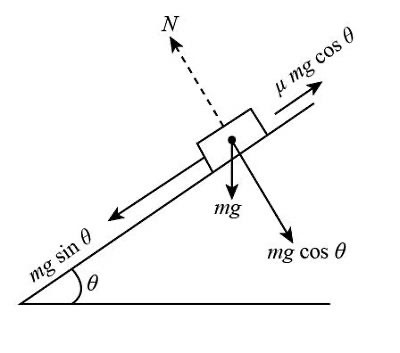
\includegraphics[width=0.5\linewidth]{../images/Piano inclinato.jpeg}
\end{figure}
\noindent
\subsection{Lavoro meccanico}

\noindent
Il lavoro meccanico misura l'energia trasferita da una forza che provoca uno spostamento.

\[
\boxed{L=Fs\cos\theta}
\]

\noindent
dove:

\begin{itemize}
    \item $L$ = lavoro (J)
    \item $F$ = forza applicata (N)
    \item $s$ = spostamento (m)
    \item $\theta$ = angolo tra forza e spostamento
\end{itemize}

\noindent
Il lavoro è:

\begin{itemize}
    \item positivo se la forza favorisce il moto;
    \item nullo se la forza è perpendicolare allo spostamento;
    \item negativo se la forza si oppone al moto.
\end{itemize}

\vspace{0.3cm}

\subsection{Energia cinetica}

\noindent
L'energia cinetica è l'energia posseduta da un corpo in movimento.

\[
\boxed{E_c=\frac12 mv^2}
\]

\noindent
dove:

\begin{itemize}
    \item $E_c$ = energia cinetica (J)
    \item $m$ = massa (kg)
    \item $v$ = velocità (m/s)
\end{itemize}

\noindent
L'energia cinetica aumenta con il quadrato della velocità.

\vspace{0.3cm}

\subsection{Teorema lavoro-energia}

\noindent
Il lavoro della forza risultante è uguale alla variazione dell'energia cinetica.

\[
\boxed{L=\Delta E_c}
\]

\[
\boxed{L=E_{c,f}-E_{c,i}}
\]

\noindent
dove:

\begin{itemize}
    \item $E_{c,i}$ = energia cinetica iniziale
    \item $E_{c,f}$ = energia cinetica finale
\end{itemize}

\noindent
Questa relazione deriva dalla seconda legge di Newton e dalle equazioni della cinematica.

\vspace{0.3cm}

\subsection{Energia potenziale gravitazionale}

\noindent
L'energia potenziale gravitazionale rappresenta l'energia che un corpo possiede a causa della sua posizione nel campo gravitazionale terrestre.

\[
\boxed{E_p=mgh}
\]

\noindent
dove:

\begin{itemize}
    \item $E_p$ = energia potenziale gravitazionale (J)
    \item $m$ = massa (kg)
    \item $g=9.81\ \mathrm{m/s^2}$
    \item $h$ = altezza rispetto al livello di riferimento (m)
\end{itemize}

\noindent
Maggiore è l'altezza, maggiore è l'energia potenziale.

\vspace{0.3cm}

\subsection{Conservazione dell'energia meccanica}

\noindent
L'energia meccanica è la somma di energia cinetica ed energia potenziale.

\[
\boxed{E_m=E_c+E_p}
\]

\noindent
Se sono presenti soltanto forze conservative (ad esempio la forza peso), l'energia meccanica si conserva.

\[
\boxed{E_{c,i}+E_{p,i}=E_{c,f}+E_{p,f}}
\]

\noindent
Durante la caduta:

\begin{itemize}
    \item l'energia potenziale diminuisce;
    \item l'energia cinetica aumenta;
    \item la loro somma rimane costante.
\end{itemize}

\vspace{0.3cm}

\subsection{Potenza}

\noindent
La potenza misura la rapidità con cui viene compiuto un lavoro.

\[
\boxed{P=\frac{L}{\Delta t}}
\]

\noindent
dove:

\begin{itemize}
    \item $P$ = potenza (W)
    \item $L$ = lavoro (J)
    \item $\Delta t$ = intervallo di tempo (s)
\end{itemize}

\noindent
L'unità di misura della potenza è il Watt.

\[
1\ W=1\ \frac{J}{s}
\]

\vspace{0.3cm}

\noindent
Se la forza è costante e parallela alla velocità, la potenza può essere calcolata anche come:

\[
\boxed{P=Fv}
\]

\noindent
dove:

\begin{itemize}
    \item $F$ = forza (N)
    \item $v$ = velocità (m/s)
\end{itemize}

\vspace{0.3cm}
\section{Gravitazione}

\subsection{Legge di gravitazione universale}

\noindent Due corpi dotati di massa si attraggono con una forza direttamente proporzionale al prodotto delle loro masse e inversamente proporzionale al quadrato della distanza che li separa.

\[
F=G\frac{m_1m_2}{r^2}
\]

\noindent dove:
\[
G=\text{costante di gravitazione universale}
\]

\[
m_1,m_2=\text{masse dei due corpi}
\]

\[
r=\text{distanza tra i centri delle masse}
\]

\vspace{0.3cm}

\noindent L'accelerazione di gravità sulla superficie terrestre vale:

\[
g=G\frac{M}{R^2}
\]

\noindent dove:

\[
M=\text{massa della Terra}
\]

\[
R=\text{raggio terrestre}
\]

\vspace{0.3cm}

\noindent Il peso di un corpo è una particolare forza gravitazionale:

\[
P=mg
\]

\vspace{0.5cm}

\subsection{Velocità orbitale}

\noindent Per un satellite in orbita circolare la forza gravitazionale coincide con la forza centripeta.

\[
G\frac{Mm}{r^2}=\frac{mv^2}{r}
\]

\noindent Da cui si ricava:

\[
v_o=\sqrt{\frac{GM}{r}}
\]

\noindent Più il satellite è vicino alla Terra, maggiore sarà la sua velocità orbitale.

\vspace{0.5cm}

\subsection{Velocità di fuga}

\noindent La velocità di fuga è la velocità minima necessaria affinché un corpo riesca ad allontanarsi definitivamente dal campo gravitazionale terrestre.

\[
v_f=\sqrt{\frac{2GM}{r}}
\]

\noindent Vale inoltre la relazione:

\[
v_f=\sqrt{2}\,v_o
\]

\vspace{0.3cm}

\noindent Possibili casi:

\begin{itemize}
\item $v<v_o$ : il satellite ricade sulla Terra.
\item $v=v_o$ : orbita circolare.
\item $v_o<v<v_f$ : orbita ellittica.
\item $v=v_f$ : il satellite sfugge con velocità finale nulla.
\item $v>v_f$ : il satellite sfugge mantenendo una velocità residua.
\end{itemize}

\vspace{0.5cm}

\section{Moto armonico semplice}

\subsection{Oscillazioni}

\noindent Il moto armonico semplice è un moto oscillatorio periodico attorno ad una posizione di equilibrio.

\vspace{0.3cm}

\noindent Le grandezze principali sono:

\begin{itemize}
\item ampiezza $A$;
\item periodo $T$;
\item frequenza $f$.
\end{itemize}

\vspace{0.3cm}

\noindent La frequenza è il numero di oscillazioni compiute in un secondo.

\[
f=\frac{1}{T}
\]

\noindent oppure

\[
T=\frac{1}{f}
\]

\vspace{0.3cm}

\noindent L'ampiezza è la massima distanza dalla posizione di equilibrio.

\vspace{0.5cm}

\subsection{Legge di Hooke}

\noindent La forza elastica esercitata da una molla è:

\[
F=-kx
\]

\noindent dove:

\[
k=\text{costante elastica}
\]

\[
x=\text{spostamento dalla posizione di equilibrio}
\]

\vspace{0.3cm}

\noindent Il segno negativo indica che la forza elastica è sempre diretta verso la posizione di equilibrio.

\vspace{0.3cm}

\noindent Dalla seconda legge di Newton:

\[
F=ma
\]

\noindent si ottiene:

\[
ma=-kx
\]

\noindent quindi:

\[
a=-\frac{k}{m}x
\]

\vspace{0.3cm}

\noindent L'accelerazione è:

\begin{itemize}
\item proporzionale allo spostamento;
\item opposta allo spostamento;
\item diretta verso l'equilibrio.
\end{itemize}

\vspace{0.5cm}

\subsection{Massa collegata ad una molla}

\noindent Nei punti di massima elongazione:

\begin{itemize}
\item velocità nulla;
\item forza elastica massima;
\item accelerazione massima.
\end{itemize}

\vspace{0.3cm}

\noindent Nella posizione di equilibrio:

\begin{itemize}
\item velocità massima;
\item forza elastica nulla;
\item accelerazione nulla.
\end{itemize}

\vspace{0.5cm}

\subsection{Pendolo semplice}

\noindent Il pendolo semplice è costituito da una massa appesa ad un filo inestensibile.

\vspace{0.3cm}

\noindent Per piccole oscillazioni il periodo vale:

\[
T=2\pi\sqrt{\frac{L}{g}}
\]

\noindent dove:

\[
L=\text{lunghezza del filo}
\]

\[
g=\text{accelerazione di gravità}
\]

\vspace{0.3cm}

\noindent Osservazioni:

\begin{itemize}
\item aumentando la lunghezza del filo aumenta il periodo;
\item aumentando la gravità diminuisce il periodo;
\item il periodo non dipende dalla massa;
\item per piccole oscillazioni non dipende dall'ampiezza.
\end{itemize}
\chapter{Fluidi e Termodinamica}

\section{Fluidi}

\subsection{Densità}

La densità rappresenta la massa contenuta in un'unità di volume.

\[
\rho=\frac{m}{V}
\]

\noindent dove:

\begin{itemize}
    \item $\rho$ = densità ($kg/m^3$);
    \item $m$ = massa;
    \item $V$ = volume.
\end{itemize}

\noindent Maggiore è la densità, maggiore è la massa contenuta nello stesso volume.

\subsection{Pressione}

La pressione misura la forza esercitata per unità di superficie.

\[
P=\frac{F}{A}
\]

\noindent dove:

\begin{itemize}
    \item $P$ = pressione (Pa);
    \item $F$ = forza (N);
    \item $A$ = area ($m^2$).
\end{itemize}

\noindent L'unità di misura della pressione è il Pascal.

\[
1\ Pa=1\ \frac{N}{m^2}
\]

\subsection{Legge di Stevino}

La pressione in un fluido aumenta con la profondità.

\[
P=\rho gh
\]

\noindent dove:

\begin{itemize}
    \item $\rho$ = densità del fluido;
    \item $g$ = accelerazione di gravità;
    \item $h$ = profondità.
\end{itemize}

\noindent La pressione dipende solamente da:

\begin{itemize}
    \item densità del fluido;
    \item accelerazione di gravità;
    \item profondità.
\end{itemize}

\noindent Non dipende dalla forma del recipiente (Paradosso Idrostatico).

\subsection{Pressione assoluta}

La pressione assoluta è la somma della pressione atmosferica e della pressione idrostatica.

\[
P_{ass}=P_{atm}+\rho gh
\]

\noindent dove:

\begin{itemize}
    \item $P_{ass}$ = pressione assoluta;
    \item $P_{atm}$ = pressione atmosferica.
\end{itemize}

\subsection{Principio di Pascal}

Una variazione di pressione applicata ad un fluido incomprimibile si trasmette inalterata in ogni punto del fluido.

\[
\frac{F_1}{A_1}=\frac{F_2}{A_2}
\]

\noindent Da cui:

\[
F_2=F_1\frac{A_2}{A_1}
\]

\noindent Osservazioni:

\begin{itemize}
    \item la pressione rimane costante;
    \item aumentando l'area del pistone aumenta la forza;
    \item aumentando la forza diminuisce lo spostamento;
    \item la pressa idraulica non crea energia.
\end{itemize}

\noindent Il lavoro rimane costante.

\[
L=Fs
\]

\subsection{Principio di Archimede}

Un corpo immerso totalmente o parzialmente in un fluido riceve una forza diretta verso l'alto pari al peso del fluido spostato.

\[
F_A=\rho gV
\]

\noindent dove:

\begin{itemize}
    \item $F_A$ = spinta di Archimede;
    \item $\rho$ = densità del fluido;
    \item $g$ = accelerazione di gravità;
    \item $V$ = volume immerso.
\end{itemize}

\subsection{Galleggiamento}

Confrontando il peso con la spinta di Archimede si hanno tre possibili casi:

\begin{itemize}
    \item $F_A=P$ : il corpo galleggia;
    \item $P>F_A$ : il corpo affonda;
    \item $F_A>P$ : il corpo sale fino alla superficie.
\end{itemize}

In generale:

\begin{itemize}
    \item se $\rho_{corpo}<\rho_{fluido}$ il corpo galleggia;
    \item se $\rho_{corpo}>\rho_{fluido}$ il corpo affonda;
    \item se $\rho_{corpo}=\rho_{fluido}$ il corpo rimane in equilibrio.
\end{itemize}

\subsection{Perché una nave galleggia}

Una nave è costruita in acciaio ma è cava al suo interno.

\noindent L'aria aumenta il volume molto più della massa, quindi la densità media della nave diventa minore di quella dell'acqua.

\noindent Per questo motivo la nave galleggia.

\noindent Un chiodo, invece, è completamente pieno di acciaio, ha densità maggiore di quella dell'acqua e quindi affonda.

\section{Temperatura e Calore}

\subsection{Temperatura}

La temperatura misura il grado di agitazione termica media delle particelle di un corpo.

\subsection{Calore}

Il calore è l'energia che si trasferisce spontaneamente da un corpo a temperatura maggiore ad uno a temperatura minore.

\subsection{Scala Kelvin}

Conversione tra Celsius e Kelvin:

\[
T(K)=T(^{\circ}C)+273.15
\]

\noindent dove:

\begin{itemize}
    \item $T(K)$ = temperatura in Kelvin;
    \item $T(^{\circ}C)$ = temperatura in gradi Celsius.
\end{itemize}

\subsection{Calore specifico}

Il calore specifico è la quantità di calore necessaria per aumentare di $1^\circ C$ (o $1\,K$) la temperatura di $1\,kg$ di sostanza.

\noindent L'unità di misura è:

\[
\frac{J}{kg\cdot K}
\]

\vspace{0.3cm}

\subsection{Calore sensibile}

Formula fondamentale:

\[
Q=mc\Delta T
\]

\noindent dove:

\begin{itemize}
    \item $Q$ = calore scambiato $(J)$;
    \item $m$ = massa $(kg)$;
    \item $c$ = calore specifico $\left(\frac{J}{kg\cdot K}\right)$;
    \item $\Delta T=T_f-T_i$ = variazione di temperatura.
\end{itemize}

\subsection{Segno del calore}

\begin{itemize}
    \item $Q>0$ : il corpo assorbe calore.
    \item $Q<0$ : il corpo cede calore.
\end{itemize}

\vspace{0.3cm}

\subsection{Osservazioni}

\begin{itemize}
    \item Maggiore è la massa, maggiore è il calore necessario.
    \item Maggiore è il calore specifico, maggiore è il calore necessario.
    \item Maggiore è la variazione di temperatura, maggiore è il calore necessario.
\end{itemize}

\section{Cambiamenti di stato}

Durante un cambiamento di stato la temperatura rimane costante.

\noindent Il calore fornito o ceduto viene utilizzato esclusivamente per cambiare lo stato fisico della sostanza.

\vspace{0.3cm}

\subsection{Calore latente}

Formula:

\[
Q=mL
\]

\noindent dove:

\begin{itemize}
    \item $Q$ = calore scambiato $(J)$;
    \item $m$ = massa $(kg)$;
    \item $L$ = calore latente $\left(\frac{J}{kg}\right)$.
\end{itemize}

\subsection{Tipi di calore latente}

\begin{itemize}
    \item Calore latente di fusione ($L_f$): passaggio da solido a liquido.
    \item Calore latente di solidificazione: passaggio da liquido a solido.
    \item Calore latente di vaporizzazione ($L_v$): passaggio da liquido a vapore.
    \item Calore latente di condensazione: passaggio da vapore a liquido.
\end{itemize}

\subsection{Attenzione}

Durante:

\begin{itemize}
    \item la fusione;
    \item l'ebollizione;
    \item la solidificazione;
    \item la condensazione;
\end{itemize}

\noindent la temperatura rimane costante fino al completamento del cambiamento di stato.

\vspace{0.3cm}
\section{Primo principio della termodinamica}

\subsection{Sistema termodinamico}

\noindent Un sistema termodinamico è la porzione di universo oggetto di studio.

\noindent Può scambiare con l'ambiente:

\begin{itemize}
    \item calore;
    \item lavoro.
\end{itemize}

\vspace{0.3cm}

\subsection{Energia interna}

\noindent L'energia interna è l'energia microscopica posseduta dalle molecole del sistema.

\noindent Si indica con:

\[
U
\]

\noindent Generalmente interessa la sua variazione:

\[
\Delta U
\]

\vspace{0.3cm}

\subsection{Primo principio della termodinamica}

\noindent L'energia non si crea né si distrugge, ma si trasforma.

\[
\Delta U=Q-L
\]

\noindent dove:

\begin{itemize}
    \item $\Delta U$ = variazione dell'energia interna;
    \item $Q$ = calore scambiato dal sistema;
    \item $L$ = lavoro compiuto dal sistema.
\end{itemize}

\vspace{0.3cm}

\noindent Convenzione dei segni:

\begin{itemize}
    \item $Q>0$ : il sistema assorbe calore;
    \item $Q<0$ : il sistema cede calore;
    \item $L>0$ : il sistema compie lavoro;
    \item $L<0$ : il lavoro viene compiuto sul sistema.
\end{itemize}

\vspace{0.3cm}

\noindent\textbf{Osservazione}

\noindent Se il gas si espande compie lavoro e la sua energia interna diminuisce.

\noindent Se il gas viene compresso, il lavoro è compiuto sul sistema e la sua energia interna aumenta.

\vspace{0.3cm}

\section{Trasformazioni termodinamiche}

\subsection{Trasformazione isocora}

\noindent Il volume rimane costante.

\[
V=\text{costante}
\]

\noindent Il lavoro è nullo.

\[
L=0
\]

\noindent Il Primo Principio diventa:

\[
\Delta U=Q
\]

\vspace{0.3cm}

\subsection{Trasformazione isobara}

\noindent La pressione rimane costante.

\[
P=\text{costante}
\]

\noindent Il volume varia e il sistema compie lavoro.

\[
L\neq0
\]

\noindent Il Primo Principio rimane:

\[
\Delta U=Q-L
\]

\vspace{0.3cm}

\subsection{Trasformazione isoterma}

\noindent La temperatura rimane costante.

\[
T=\text{costante}
\]

\noindent Per un gas ideale:

\[
\Delta U=0
\]

\noindent Quindi:

\[
Q=L
\]

\vspace{0.3cm}

\subsection{Trasformazione adiabatica}

\noindent Non avviene alcuno scambio di calore.

\[
Q=0
\]

\noindent Il Primo Principio diventa:

\[
\Delta U=-L
\]

\vspace{0.3cm}

\noindent\textbf{Osservazioni}

\begin{itemize}
    \item Se il gas si espande, la temperatura diminuisce.
    \item Se il gas viene compresso, la temperatura aumenta.
\end{itemize}

\vspace{0.3cm}

\subsection{Schema riassuntivo}

\begin{center}
\begin{tabular}{|c|c|c|}
\hline
Trasformazione & Grandezza costante & Relazione principale \\
\hline
Isocora & Volume & $L=0$ \\
\hline
Isobara & Pressione & $\Delta U=Q-L$ \\
\hline
Isoterma & Temperatura & $\Delta U=0,\;Q=L$ \\
\hline
Adiabatica & $Q=0$ & $\Delta U=-L$ \\
\hline
\end{tabular}
\end{center}

\vspace{0.3cm}

\section{Secondo principio della termodinamica}

\noindent Il calore passa spontaneamente dal corpo a temperatura maggiore al corpo a temperatura minore.

\vspace{0.3cm}

\noindent All'equilibrio termico i due corpi raggiungono la stessa temperatura.

\vspace{0.3cm}

\noindent\textbf{Osservazione}

\noindent Non è possibile trasformare completamente il calore assorbito in lavoro.

\vspace{0.3cm}

\section{Macchine termiche}

\noindent Una macchina termica trasforma una parte del calore assorbito in lavoro.

\vspace{0.3cm}

\noindent Riceve:

\begin{itemize}
    \item calore dalla sorgente calda ($Q_h$);
    \item cede calore alla sorgente fredda ($Q_c$);
    \item produce lavoro ($L$).
\end{itemize}

\noindent Vale la relazione:

\[
Q_h=L+Q_c
\]

\vspace{0.3cm}

\subsection{Rendimento}

\noindent Il rendimento rappresenta l'efficienza della macchina termica.

\[
\eta=\frac{L}{Q_h}
\]

\noindent oppure

\[
\eta=1-\frac{Q_c}{Q_h}
\]

\noindent dove:

\begin{itemize}
    \item $\eta$ = rendimento;
    \item $L$ = lavoro prodotto;
    \item $Q_h$ = calore assorbito dalla sorgente calda;
    \item $Q_c$ = calore ceduto alla sorgente fredda.
\end{itemize}

\vspace{0.3cm}

\noindent\textbf{Condizione}

\[
0<\eta<1
\]

\noindent oppure

\[
0\%<\eta<100\%
\]

\vspace{0.3cm}

\noindent Nessuna macchina termica reale può avere rendimento pari al $100\%$.

\vspace{0.3cm}

\section{Macchina di Carnot}

\noindent La macchina di Carnot è una macchina termica ideale che possiede il massimo rendimento teoricamente possibile.

\vspace{0.3cm}

\noindent Il rendimento vale:

\[
\eta=1-\frac{T_f}{T_c}
\]

\noindent dove:

\begin{itemize}
    \item $T_c$ = temperatura della sorgente calda;
    \item $T_f$ = temperatura della sorgente fredda.
\end{itemize}

\vspace{0.3cm}

\noindent\textbf{Attenzione}

\noindent Le temperature devono essere sempre espresse in Kelvin.

